\section{Vectors} \label{S:9.2.Vectors}


\vspace*{-14 pt}
\framebox{\hspace*{3 pt}
\parbox{6.25 in}{\begin{goals}
\item What is a vector?
\item What does it mean for two vectors to be equal?
\item How do we add two vectors together and multiply a vector by a scalar?
\item How do we determine the magnitude of a vector?  What is a unit vector, and how do we find a unit vector in the direction of a given vector?
\end{goals}} \hspace*{3 pt}}

\subsection*{Introduction}

If we are at a point $x$ in the domain of a function of one variable,
there are only two directions in which we can move: in the positive or
negative $x$-direction. If, however, we are at a point $(x,y)$ in the domain of
a function of two variables, there are many
directions in which we can move. Thus, it is important for us to have
a means to indicate direction, and we will do so using vectors.

\begin{pa} \label{PA:9.2}
After working out, Sarah and John leave the Recreation Center on the Grand Valley State University Allendale campus (a map of which is given in Figure \ref{F:9.2.GVSU}) to go to their next classes.\footnote{GVSU campus map from \url{http://www.gvsu.edu/homepage/files/pdf/maps/allendale.pdf}, used with permission from GVSU, credit to illustrator Chris Bessert.}  Suppose we record Sarah's movement on the map in a pair $\langle x, y \rangle$ (we will call this pair a \emph{vector}), where $x$ is the horizontal distance (in feet) she moves (with east as the positive direction) and $y$ as the vertical distance (in feet) she moves (with north as the positive direction). We do the same for John. Throughout, use the legend to estimate your responses as best you can. 

    \ba
   \item What is the vector $\vv_1 = \langle x , y \rangle$ that describes Sarah's movement if she walks directly in a straight line path from the Recreation Center to the entrance at the northwest end of Mackinac Hall? (Assume a straight line path, even if there are buildings in the way.) Explain how you found this vector. What is the total distance in feet between the Recreation Center and the entrance to Mackinac Hall?  Measure the number of feet directly and then explain how to calculate this distance in terms of $x$ and $y$.



    \item What is the vector $\vv_2 = \langle x , y \rangle$ that describes John's change in position if he walks directly from the Recreation Center to Au Sable Hall? How many feet are there between Recreation Center to Au Sable Hall in terms of $x$ and $y$?



    \item What is the vector $\vv_3 = \langle x , y \rangle$ that describes the change in position if John walks directly from Au Sable Hall to the northwest entrance of Mackinac Hall to meet up with Sarah after class? What relationship do you see among the vectors $\vv_1$, $\vv_2$, and $\vv_3$? Explain why this relationship should hold.



	\ea


\end{pa} 

\begin{activitySolution}
    \ba
   \item Using a marked straightedge, the horizontal distance from the Recreation Center to the entrance at the northwest end of Mackinac Hall is approximately 750 feet, while the vertical distance is about 420 feet. Since Sarah traveled east and north, the vector describing her movement is ${\vv_1 = \langle 750, 420 \rangle}$. The straight line distance from the Recreation Center to the entrance at the northwest end of Mackinac Hall is measured with straightedge as approximately 875 feet, and this can be found using the Pythagorean Theorem on the right triangle with $x$ and $y$ as legs and the distance from the Recreation Center to the entrance at the northwest end of Mackinac Hall as the hypotenuse. This gives the straight line distance from the Recreation Center to the entrance at the northwest end of Mackinac Hall as
\[\sqrt{(750)^2 + (420)^2} \approx 859.6 \text{ feet}.\]
Of course, there is error here in all of the measurements.

    \item Using a marked straightedge, the horizontal distance from the Recreation Center to Au Sable Hall is approximately 1200 feet, while the vertical distance is about 1100 feet. Since John traveled east and south, the vector describing his movement is ${\vv_2 = \langle 1200, -1100 \rangle}$. John walked approximately
\[\sqrt{1200^2 + (-1100)^2} \approx 1627.88 \text{ feet}.\]


    \item Using a marked straightedge, the horizontal distance from Au Sable Hall to the northwest entrance of Mackinac is approximately 450 feet, while the vertical distance is about 1520 feet. Since John traveled west and north, the vector describing this movement is ${\vv_3 = \langle -450, 15205 \rangle}$. The horizontal distance traveled from Au Sable Hall to the northwest entrance of Mackinac is the difference of the distances from the Recreation Center to Au Sable Hall and from the Recreation Center to the northwest entrance of Mackinac (this is because John traveled in opposite horizontal directions), while the vertical distance from Au Sable Hall to the northwest entrance of Mackinac is the sum of the vertical distance from the Recreation Center to the northwest entrance of Mackinac and the vertical distance from the Recreation Center to Au Sable Hall (since John travels in the vertical direction). So, in essence,
\[\vv_3 = \vv_1 - \vv_2.\]


	\ea

\end{activitySolution}

\afterpa 

%\newpage

\begin{figure}[ht]
\begin{center}
\resizebox{!}{5.9in}{\includegraphics{figures/9_2_GVSU_map.pdf}}
%\resizebox{!}{6.0in} [height=6.5in, width=5.0in] trim left bottom right top [trim=0.1cm 0.5cm 01.cm 0.5cm, clip]
\end{center}
\caption{Grand Valley State University Allendale campus map.} 
\label{F:9.2.GVSU}
\end{figure}

%\newpage

\subsection*{Representations of Vectors}

Preview Activity \ref{PA:9.2} shows how we can record the magnitude
and direction of a change in position using an ordered pair of numbers
$\langle x,y\rangle$. There are many other quantities, such as force
and velocity, that possess the attributes of magnitude and direction,
and we will call each such quantity a {\em vector}.

\vspace*{5pt}
\nin \framebox{\hspace*{3 pt}
  \parbox{6.25 in}{\begin{definition} A
      \textbf{vector}\index{vector!definition} is any quantity
      that possesses the attributes of magnitude and
      direction. \end{definition} } \hspace*{3 pt}} \vspace*{5pt}

We can represent a vector geometrically as a directed line segment,
with the magnitude as the length of the segment and an arrowhead
indicating direction, as shown in Figure \ref{F:9.2.vectors.single}.

\begin{figure}[ht]
  \begin{center}
    \begin{minipage}{2.5in}
      \begin{center}
        % \resizebox{!}{1.75in}{\includegraphics{9_2_Vector1}}
        % fig1.15.py
        \includegraphics{figures/fig_9_2_single.eps}
      \end{center}
      \caption{A vector.}
      \label{F:9.2.vectors.single}
    \end{minipage}
    \begin{minipage}{3.3in}
      \begin{center}
        % \resizebox{!}{1.75in}{\includegraphics{9_2_Vector1}}
        % fig1.15.a.py
        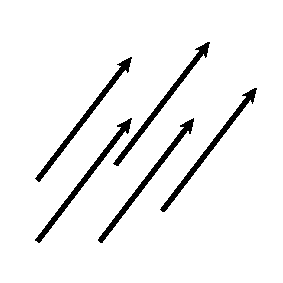
\includegraphics{figures/fig_9_2_multiple.eps}
      \end{center}
      \caption{Representations of the same vector.}
      \label{F:9.2.vectors.many}
    \end{minipage}
  \end{center}
\end{figure}


According to the definition, a vector possesses the attributes of
length (magnitude) and direction; the vector's position, however, is
not mentioned.  Consequently, we regard as equal any two vectors having the
same magnitude and direction, as shown in Figure
\ref{F:9.2.vectors.many}.

\vspace*{5pt}
\nin 
\begin{center}
  \framebox{
    \parbox{5.25 in}{ 
      \hfill
      Two vectors are equal provided they have the
      same magnitude and direction.  
      \hfill
    }
  }
\end{center}
\vspace*{5pt}

This means that the same vector may be drawn in the plane in many
different ways.  For instance, suppose that we would like to draw the
vector $\langle 3, 4\rangle$, which
represents a horizontal
change of three units and a vertical change of four units.
We may place the \emph{tail} of the vector (the point from which the
vector originates) at the origin and the \emph{tip} (the terminal
point of the vector) at $(3,4)$, as illustrated in Figure
\ref{F:9.2.vectors2}.  A vector with its tail at the origin is
said to be in \emph{standard position}.

\begin{figure}[ht]
  \begin{center}
    \begin{minipage}{3.0in}
      \begin{center}
        % \resizebox{!}{1.75in}{\includegraphics{9_2_Vector2}}
        % fig1.15.py
%        \includegraphics{figures/fig-9-16.eps}
        \includegraphics{figures/fig_9_2_std_pos.eps}
      \end{center}
      \caption{A vector in standard position}
      \label{F:9.2.vectors2}
    \end{minipage}
    \begin{minipage}{3.0in}
      \begin{center}
        % \resizebox{!}{1.75in}{\includegraphics{9_2_Vector3}}
        % fig1.15.py
%        \includegraphics{figures/fig-9-17.eps}
        \includegraphics{figures/fig_9_2_btw_pts.eps}
      \end{center}
      \caption{A vector between two points}
      \label{F:9.2.vectors3}
    \end{minipage}
  \end{center}
\end{figure}

Alternatively, we may place the tail of the vector $\langle
3,4\rangle$ at another point, such as $Q(1,1)$.  After a displacement
of three units to the right and four units up, the tip of
the vector is at the point $R(4,5)$ (see
Figure \ref{F:9.2.vectors3}).

In this example, the vector led to the directed line segment from $Q$
to $R$, which we denote as $\overrightarrow{QR}$.  We may also
turn the situation around: given the two points $Q$ and $R$, we obtain
the vector $\langle 3,4\rangle$ because we move horizontally three
units and vertically four units to get from $Q$ to $R$.  In other
words, $\overrightarrow{QR} = \langle 3,4\rangle$.  In general, the
vector $\overrightarrow{QR}$ from the point $Q = (q_1, q_2)$ to $R = (r_1,
r_2)$ is found by taking the difference of coordinates, so that
\[\overrightarrow{QR} = \langle r_1-q_1, r_2-q_2 \rangle.\]

We will use boldface letters to represent vectors, such
as $\vv = \langle 3, 4 \rangle$, to distinguish them from scalars. The
entries of a vector are called its \emph{components}; in the vector
$\langle 3, 4 \rangle$, the $x$ component is 3 and the $y$
component is 4. We use pointed brackets $\langle \ , \rangle$ and the term
\emph{components} to distinguish a vector from a point $( \ , )$ and
its \emph{coordinates}.  There is, however, a close connection between vectors
and points.  Given a point $P$, we will frequently consider the vector
$\overrightarrow{OP}$ from the origin $O$ to $P$.  For instance, if
$P=(3,4)$, then $\overrightarrow{OP}=\langle 3,4\rangle$ as in Figure \ref{F:9.2.vectors4}.  
In this way, we think of a point $P$ as defining a vector
$\overrightarrow{OP}$ whose components agree with the coordinates of
$P$.

\begin{figure}[ht]
  \begin{center}
%    \includegraphics{figures/fig-9-15-b.eps}
    \includegraphics{figures/fig_9_2_pt_def.eps}
      \caption{A point defines a vector}
      \label{F:9.2.vectors4}    

  \end{center}
\end{figure}

While we often illustrate vectors in the plane since it is easier
to draw pictures, different situations call for the use of vectors
in three or more dimensions.  For instance, a
vector $\vv$ in $n$-dimensional space, $\R^n$, has $n$
components and may be represented as
\[\vv = \langle v_1, v_2, v_3,  \ldots, v_n \rangle.\]

The next activity will help us to become accustomed to vectors and
operations on vectors in three dimensions.

\begin{activity} \label{A:9.2.1}  As a class, determine a coordinatization of your classroom, agreeing on some convenient set of axes (e.g., an intersection of walls and floor) and some units in the $x$, $y$, and $z$ directions (e.g., using lengths of sides of floor, ceiling, or wall tiles). Let $O$ be the origin of your coordinate system. Then, choose three points, $A$, $B$, and $C$ in the room, and complete the following.
\ba
	\item Determine the coordinates of the points $A$, $B$, and $C$.

    \item Determine the components of the indicated vectors.
    \begin{center}
	\begin{tabular}{cccccc}
(i) $\overrightarrow{OA}$ &(ii) $\overrightarrow{OB}$ &(iii) $\overrightarrow{OC}$ &(iv) $\overrightarrow{AB}$ &(v) $\overrightarrow{AC}$ &(vi) $\overrightarrow{BC}$
	\end{tabular}
    \end{center}

    \ea
\end{activity}
\begin{smallhint}

\end{smallhint}
\begin{bighint}

\end{bighint}
\begin{activitySolution}

\end{activitySolution}
\aftera


\subsection*{Equality of Vectors}

Because location is not mentioned in the
definition of a vector, any two vectors that have the same
magnitude and direction are equal. It is helpful to have an
algebraic way to determine when this occurs. That is, if we know the
components of two vectors $\vu$ and $\vv$, we will want to be able to
determine algebraically when $\vu$ and $\vv$ are equal. There is an
obvious set of conditions that we use.

%\begin{activity}  \label{A:9.2.2}
    \ba
    \item In terms of the components, how can we tell if two vectors $\vu = \langle u_1, u_2 \rangle$ and $\vv = \langle v_1, v_2 \rangle$ in $\R^2$ are equal? Explain your reasoning.

    \item In terms of the components, how can we tell if two vectors $\vu = \langle u_1, u_2, u_3\rangle$ and $\vv = \langle v_1, v_2, v_3 \rangle$ in $\R^3$ are equal? Explain your reasoning.


    \ea

\end{activity}
\begin{smallhint}
\ba
\item How can $\vu$ and $\vv$ in $\R^2$ have the same direction and magnitude? 
\item How can $\vu$ and $\vv$ in $\R^2$ have the same direction and magnitude? 
\ea
\end{smallhint}
\begin{bighint}
\ba
\item What does it mean for two points $(u_1,u_2)$ and $(v_1,v_2)$ to be equal? 
\item What does it mean for two points $(u_1,u_2, u_3)$ and $(v_1,v_2,v_3)$ to be equal? 
\ea
\end{bighint}
\begin{activitySolution}
\ba
\item For two vectors to be equal, the vectors should have the same direction and magnitude. For vectors $\vu = \langle u_1, u_2 \rangle$ and $\vv = \langle v_1, v_2 \rangle$ in $\R^2$ this will happen when $u_1=v_1$ and $u_2=v_2$.
\item For two vectors to be equal, the vectors should have the same direction and magnitude. For vectors $\vu = \langle u_1, u_2, u_3\rangle$ and $\vv = \langle v_1, v_2, v_3 \rangle$ in $\R^3$ this will happen when $u_1=v_1$, $u_2=v_2$, and $u_3=v_3$.
\ea
\end{activitySolution}
\aftera


\vspace*{5pt}
\nin \framebox{\hspace*{3 pt}
  \parbox{6.25 in}{Two vectors $\vu = \langle u_1, u_2 \rangle$ and $\vv = \langle v_1, v_2 \rangle$ in $\R^2$ are equal if and only if their corresponding components are equal:  $u_1 = v_1$ and $u_2 = v_2$.  More generally, two vectors $\vu = \langle u_1, u_2, \ldots, u_n\rangle$ and $\vv = \langle v_1, v_2, \ldots, v_n \rangle$ in $\R^n$ are equal if and only if $u_i = v_i$ for each possible value of $i$.
 } \hspace*{3 pt}} \vspace*{5pt}

\subsection*{Operations on Vectors}

Vectors are not numbers, but we can now represent them with components
that are real numbers. As such, we naturally wonder if it is possible
to add two vectors together, multiply two vectors, or combine vectors
in any other ways. In this section, we will study two
operations on vectors: vector addition and scalar multiplication. To
begin, we investigate a natural way to add two vectors together, as
well as to multiply a vector by a scalar.

\begin{activity} \label{A:9.2.3}
Let $\vu = \langle 2, 3 \rangle$, $\vv = \langle -1, 4 \rangle$.
    \ba
    \item Using the two specific vectors above, what is the natural way to define the vector sum $\vu + \vv$? 

    \item In general, how do you think the vector sum $\va + \vb$ of vectors $\va = \langle a_1, a_2 \rangle$ and $\vb = \langle b_1, b_2 \rangle$ in $\R^2$ should be defined? Write a formal definition of a vector sum based on your intuition.

    \item In general, how do you think the vector sum $\va + \vb$ of vectors $\va = \langle a_1, a_2, a_3 \rangle$ and $\vb = \langle b_1, b_2, b_3 \rangle$ in $\R^3$ should be defined? Write a formal definition of a vector sum based on your intuition.

    \item Returning to the specific vector $\vv = \langle -1, 4 \rangle$ given above, what is the natural way to define the scalar multiple $\frac{1}{2}\vv$? 

    \item In general, how do you think a scalar multiple of a vector $\va = \langle a_1, a_2 \rangle$ in $\R^2$ by a scalar $c$ should be defined? how about for a scalar multiple of a vector $\va = \langle a_1, a_2, a_3 \rangle$ in $\R^3$ by a scalar $c$? Write a formal definition of a scalar multiple of a vector based on your intuition.

    \ea
\end{activity}
\begin{smallhint}
   \ba
    \item Do the most obvious thing.
    \item Do the most obvious thing.
    \item Do the most obvious thing.
    \item Do the most obvious thing.
    \item Do the most obvious thing.
    \ea
\end{smallhint}
\begin{bighint}
	\ba
	\item Think about how to combine corresponding components. 
    \item Think about how to combine corresponding components. 
    \item Think about how to combine corresponding components. 
	\item How should a scalar affect each component?
	\item How should a scalar affect each component?
    \ea
\end{bighint}
\begin{activitySolution}
   \ba
    \item It would be natural to add vectors by adding their corresponding components. So we should expect $\vu + \vv$ to be the vector $\vu+\vv = \langle 2+(-1), 3+4 \rangle = \langle 1, 7\rangle$. 
    \item It would be natural to add vectors by adding their corresponding components. So we should expect the sum of vectors $\va = \langle a_1, a_2 \rangle$ and $\vb = \langle b_1, b_2 \rangle$ in $\R^2$ to be
\[\va + \vb =  \langle a_1, a_2 \rangle + \langle b_1, b_2 \rangle = \langle a_1+b_1, a_2+b_2 \rangle.\]
    \item It would be natural to add vectors by adding their corresponding components. So we should expect the sum of vectors $\va = \langle a_1, a_2, a_3 \rangle$ and $\vb = \langle b_1, b_2, b_3 \rangle$ in $\R^3$ to be
\[\va + \vb =  \langle a_1, a_2, a_3 \rangle + \langle b_1, b_2, b_3 \rangle = \langle a_1+b_1, a_2+b_2, a_3+b_3 \rangle.\]
    \item It would be natural to multiply a vector by a scalar by multiplying each component of the vector by that scalar. So the scalar multiple $\frac{1}{2}\vv$ should be defined as 
\[\frac{1}{2}\vv = \frac{1}{2}\langle -1, 4 \rangle = \left\langle -\frac{1}{2}, 2 \right\rangle.\]
    \item It would be natural to multiply a vector by a scalar by multiplying each component of the vector by that scalar. So the scalar multiple $c\langle a_1, a_2 \rangle$ in $\R^2$ should be defined as 
\[c\langle a_1, a_2 \rangle = \langle ca_1, ca_2 \rangle\]
and the scalar multiple $c\langle a_1, a_2, a_3 \rangle$ in $\R^3$ should be defined as 
\[c\langle a_1, a_2, a_3 \rangle = \langle ca_1, ca_2, ca_3 \rangle\]
    \ea
\end{activitySolution}
\aftera


%There is also a natural way to multiply a vector by a scalar (a real number).
%\input{activities/9.2.Act4}

We can now add vectors and multiply vectors by scalars, and thus we
can add together scalar multiples of vectors. This allows us to define
\emph{vector subtraction}\index{vector!subtraction}, $\vv - \vu$, as
the sum of $\vv$ and $-1$ times $\vu$, so that
\[\vv - \vu = \vv + (-1)\vu.\]

%\begin{activity} \label{A:9.2.5}

\begin{figure}[h]
  \begin{center}
    \begin{minipage}{3in}
      \begin{center}
        % \resizebox{!}{2.25in}{\includegraphics{figures/9_2_Vector_magnitude1}}
        \includegraphics{figures/fig-9-19-activity.eps}
      \end{center}
      \caption{} %$\overrightarrow{AB}$.
      \label{F:9.2.vector_activity1}
    \end{minipage}
    \begin{minipage}{3in}
      \begin{center}
        % \resizebox{!}{2.25in}{\includegraphics{figures/9_2_Vector_magnitude1}}
        \includegraphics{figures/fig-9-19-activity.eps}
      \end{center}
      \caption{} %$\overrightarrow{AB}$.
      \label{F:9.2.vector_activity2}
    \end{minipage}
  \end{center}
\end{figure}

Suppose that $\vu$ and $\vv$ are the vectors shown in Figure
\ref{F:9.2.vector_activity1}.   
	\ba
	\item On Figure \ref{F:9.2.vector_activity1}, sketch the
          vectors $\vu + \vv$, $\vv - \vu$, $2\vu$, $-2\vu$, and $-3\vv$. 
        \item What is $0\vv$?
        \item On Figure \ref{F:9.2.vector_activity2}, sketch the
          vectors $-3\vv$, $-2\vv$, $-1\vv$, $2\vv$, and $3\vv$.
        \item Give a geometric description of the set of vectors
          $t\vv$ where $t$ is any scalar.
        \item On Figure \ref{F:9.2.vector_activity2}, sketch the
          vectors $\vu-3\vv$, $\vu-2\vv$, $\vu-\vv$, $\vu + \vv$, and
          $\vu + 2\vv$.  
        \item Give a geometric description of the set of vectors
          $\vu + t\vv$ where $t$ is any scalar.

	\ea


\end{activity}
\begin{smallhint}

\end{smallhint}
\begin{bighint}

\end{bighint}
\begin{activitySolution}
	\ba
	\item A sketch of the vectors is shown below at left. 
    \item If we multiply any vector by the zero scalar, each component of the vector is multiplied by 0, resulting in the zero vector. So $0\vv = \vzero$.
    \item A sketch of the vectors is shown below at left. 
    \item This is the line through the origin in the direction of the vector $\vv$. 
     \item The vectors are shown below at right. 
\begin{center}
        \resizebox{!}{2.25in}{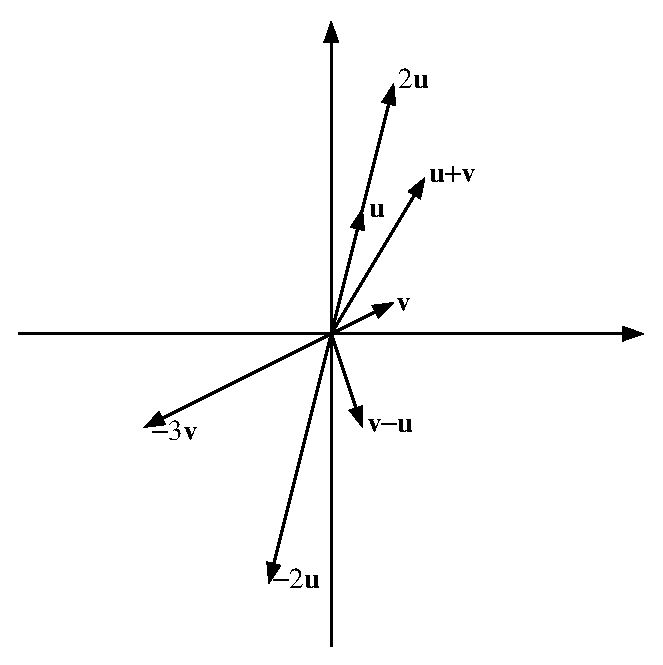
\includegraphics{figures/9_2_Act_5_Vectors_a}} \ \ \resizebox{!}{2.25in}{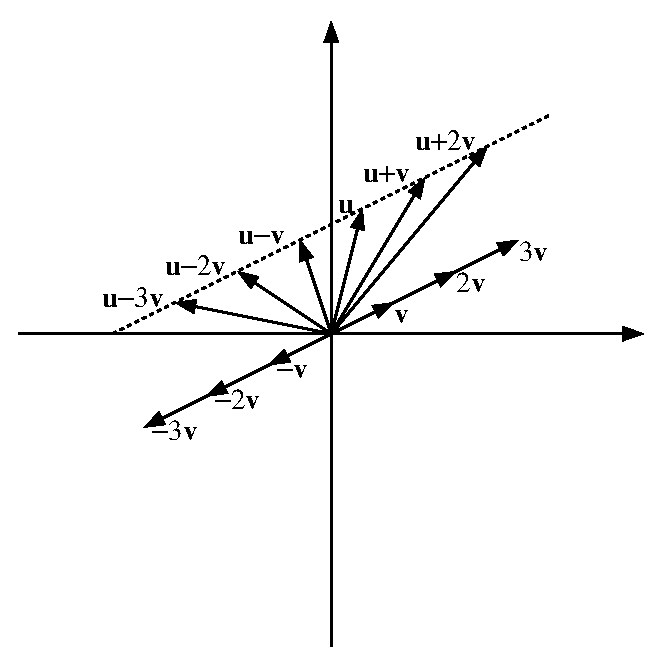
\includegraphics{figures/9_2_Act_5_Vectors_b}}
      \end{center}
     \item As the figure in part (e) illustrates, this is a line through the terminal point of the vector $\vu$ in standard position in the direction of the vector $\vv$. 
	\ea
\end{activitySolution}
\aftera



Using vector addition and scalar multiplication, we will often
represent vectors in terms of the special vectors $\vi =
\langle 1, 0 \rangle$ and $\vj = \langle 0,1 \rangle$.  For instance,
we can write 
the vector $\langle a, b \rangle$ in $\R^2$ as
\[\langle a, b \rangle = a\langle 1, 0 \rangle + b\langle 0, 1 \rangle = a\vi + b \vj,\]
which means that
\[\langle 2, -3 \rangle = 2\vi - 3\vj.\]
In the context of $\R^3$, we let $\vi = \langle 1, 0, 0 \rangle$, $\vj = \langle 0,1,0 \rangle$, and $\vk = \langle 0,0,1 \rangle$, and we can write the vector $\langle a, b, c \rangle$ in $\R^3$ as
\[\langle a, b,c \rangle = a\langle 1, 0,0 \rangle + b\langle 0, 1,0 \rangle + c\langle 0,0,1 \rangle = a\vi + b \vj + c\vk.\]
The vectors $\vi$, $\vj$, and $\vk$ are called the \emph{standard unit vectors}\footnote{As we will learn momentarily, unit vectors have length 1.}, and are important in the physical sciences.

\subsection*{Properties of Vector Operations}

We know that the scalar sum $1+2$ is equal to the scalar sum
$2+1$. This is called the \emph{commutative} property of scalar
addition. Any time we define operations on objects (like addition of
vectors) we usually want to know what kinds of properties the
operations have. For example, is addition of vectors a commutative
operation? To answer this question we take two \emph{arbitrary}
vectors $\vv$ and $\vu$ and add them together and see what
happens. Let $\vv = \langle v_1, v_2 \rangle$ and $\vu = \langle u_1,
u_2 \rangle$. Now we use the fact that $v_1$, $v_2$, $u_1$, and $u_2$
are scalars, and that the addition of scalars is commutative to see
that
\[\vv + \vu = \langle v_1, v_2 \rangle + \langle u_1, u_2 \rangle = \langle v_1+u_1, v_2 + u_2 \rangle = \langle u_1+v_1, u_2+v_2 \rangle = \langle u_1, u_2 \rangle + \langle v_1, v_2 \rangle = \vu + \vv.\]
So the vector sum is a commutative operation. Similar arguments can be
used to show the following properties of vector addition and scalar
multiplication. 

\vspace*{5pt}
\nin \framebox{\hspace*{3 pt}
\parbox{6.25 in}{Let $\vv$, $\vu$, and $\vw$ be vectors in $\R^n$ and let $a$ and $b$ be scalars. Then
\begin{enumerate}
\item $\vv + \vu = \vu + \vv$
\item $(\vv + \vu) + \vw = \vv + (\vu + \vw)$
\item The vector $\vzero = \langle 0, 0, \ldots, 0 \rangle$ has the
  property that $\vv + \vzero = \vv$. The vector $\vzero$ is called
  the \textbf{zero vector}. 
\item  $(-1)\vv + \vv = \vzero$. The vector $(-1)\vv = -\vv$ is called
  the \textbf{additive inverse} of the vector $\vv$. 
\item $(a+b) \vv = a\vv + b\vv$
\item $a(\vv + \vu) = a\vv + a\vu$
\item $(ab) \vv = a(b\vv)$
\item $1 \vv = \vv$.
\end{enumerate}
} \hspace*{3 pt}}
\vspace*{5pt}

We verified the first property for vectors in $\R^2$; it is
straightforward to verify that the rest of the eight properties just
noted hold for all 
vectors in $\R^n$. 

\subsection*{Geometric Interpretation of Vector Operations}

Next, we explore a geometric interpretation of vector addition and
scalar multiplication that allows us to visualize these operations.
Let $\vu = \langle 4, 6 \rangle$ and $\vv = \langle 3, -2
\rangle$. Then $\vw = \vu + \vv = \langle 7, 4 \rangle$, as shown on the left in
Figure \ref{F:9.2.vector_sum}.

\begin{figure}[ht]
  \begin{center}
    \includegraphics{figures/fig_9_2_operations.eps}
  \caption{A vector sum (left), summing displacements (center), the parallelogram law (right)}
  \label{F:9.2.vector_sum}
  \end{center}
\end{figure}

% \begin{figure}[ht]
% \begin{center}
% \begin{minipage}{3in}
% \begin{center}
% %\resizebox{!}{2.5in}{\includegraphics{9_2_Vector_sum1}}
% \includegraphics{figures/fig-9-18.eps}
% \end{center}
% \caption{{A vector sum}}
% \label{F:9.2.vector_sum}
% \end{minipage}
% \begin{minipage}{3in}
% \begin{center}
% %\resizebox{!}{2.5in}{\includegraphics{9_2_Vector_sum2}}
% \includegraphics{figures/fig-9-18-a.eps}
% \end{center}
% \caption{{Summing displacements}}
% \label{F:9.2.vector_sum2}
% \end{minipage}
% \end{center}
% \end{figure}

If we think of these vectors as displacements in the plane, we 
find a geometric way to envision vector addition.  For instance, the
vector $\vu + \vv$ will represent the displacement obtained by
following the displacement $\vu$ with the displacement $\vv$.  We may
picture this by placing the tail of $\vv$ at the tip of $\vu$, as seen
in the center of Figure \ref{F:9.2.vector_sum}.

Of course, vector addition is commutative so we obtain the same sum if
we place the tail of $\vu$ at the tip of $\vv$.
We therefore see that $\vu+\vv$ appears as
the 
diagonal of the
parallelogram\index{vector!sum, parallelogram} determined by $\vu$ and
$\vv$, as shown on the right of Figure \ref{F:9.2.vector_sum}. 

% \begin{figure}[ht]
% \begin{center}
% \begin{minipage}{3in}
% \begin{center}
% %\resizebox{!}{2.5in}{\includegraphics{9_2_Vector_sum1}}
% \includegraphics{figures/fig-9-18-b.eps}
% \end{center}
% \caption{{Summing displacements}}
% \label{F:9.2.vector_sum3}
% \end{minipage}
% \begin{minipage}{3in}
% \begin{center}
% %\resizebox{!}{2.5in}{\includegraphics{9_2_Vector_sum2}}
% \includegraphics{figures/fig-9-19.eps}
% \end{center}
% \caption{{$\vu$ and $\vv$} form a parallelogram}
% \label{F:9.2.vector_sum4}
% \end{minipage}
% \end{center}
% \end{figure}

Vector subtraction has a similar interpretation.  On the left in
Figure \ref{F:9.2.vector_sum5}, we see vectors $\vu$, $\vv$, and $\vw =
\vu + \vv$.  If we rewrite $\vv = \vw - \vu$, we have the arrangement
of Figure \ref{F:9.2.vector_sum6}.  In other words, to form the
difference $\vw-\vu$, we draw a vector from the tip of $\vu$ to the
tip of $\vw$. 

\begin{figure}[ht]
  \begin{center}
    \begin{minipage}{2.5in}
%    \begin{minipage}{2in}
      \begin{center}
        % \resizebox{!}{2.5in}{\includegraphics{9_2_Vector_sum1}}
%        \includegraphics{figures/fig-9-19-a.eps}
        \includegraphics{figures/fig_9_2_addition.eps}
      \end{center}
      \caption{Vector addition}
      \label{F:9.2.vector_sum5}
    \end{minipage}
    \begin{minipage}{2.5in}
%    \begin{minipage}{2in}
      \begin{center}
        % \resizebox{!}{2.5in}{\includegraphics{9_2_Vector_sum2}}
%        \includegraphics{figures/fig-9-19-b.eps}
        \includegraphics{figures/fig_9_2_subtraction.eps}
      \end{center}
      \caption{Vector subtraction}
      \label{F:9.2.vector_sum6}
    \end{minipage}
  \end{center}
\end{figure}

In a similar way, we may geometrically represent a scalar multiple of a
vector.  For instance, if $\vv=\langle 2,3\rangle$, then
$2\vv = \langle 4,6\rangle$.  As shown in Figure
\ref{F:9.2.vector_sum7}, multiplying $\vv$ by 2 leaves the direction
unchanged, but stretches $\vv$ by 2.  Also, $-2\vv = \langle -4,
-6\rangle$, which shows that multiplying by a negative scalar gives a
vector pointing in the opposite direction of $\vv$.

\newpage

\begin{figure}[ht]
  \begin{center}
    \begin{minipage}{3in}
      \begin{center}
        % \resizebox{!}{2.5in}{\includegraphics{9_2_Vector_sum1}}
%        \includegraphics{figures/fig-9-19-scalar.eps}
        \includegraphics{figures/fig_9_2_scalar.eps}
      \end{center}
      \caption{Scalar multiplication}
      \label{F:9.2.vector_sum7}
    \end{minipage}
  \end{center}
\end{figure}

\begin{activity} \label{A:9.2.5}

\begin{figure}[h]
  \begin{center}
    \begin{minipage}{3in}
      \begin{center}
        % \resizebox{!}{2.25in}{\includegraphics{figures/9_2_Vector_magnitude1}}
        \includegraphics{figures/fig-9-19-activity.eps}
      \end{center}
      \caption{} %$\overrightarrow{AB}$.
      \label{F:9.2.vector_activity1}
    \end{minipage}
    \begin{minipage}{3in}
      \begin{center}
        % \resizebox{!}{2.25in}{\includegraphics{figures/9_2_Vector_magnitude1}}
        \includegraphics{figures/fig-9-19-activity.eps}
      \end{center}
      \caption{} %$\overrightarrow{AB}$.
      \label{F:9.2.vector_activity2}
    \end{minipage}
  \end{center}
\end{figure}

Suppose that $\vu$ and $\vv$ are the vectors shown in Figure
\ref{F:9.2.vector_activity1}.   
	\ba
	\item On Figure \ref{F:9.2.vector_activity1}, sketch the
          vectors $\vu + \vv$, $\vv - \vu$, $2\vu$, $-2\vu$, and $-3\vv$. 
        \item What is $0\vv$?
        \item On Figure \ref{F:9.2.vector_activity2}, sketch the
          vectors $-3\vv$, $-2\vv$, $-1\vv$, $2\vv$, and $3\vv$.
        \item Give a geometric description of the set of vectors
          $t\vv$ where $t$ is any scalar.
        \item On Figure \ref{F:9.2.vector_activity2}, sketch the
          vectors $\vu-3\vv$, $\vu-2\vv$, $\vu-\vv$, $\vu + \vv$, and
          $\vu + 2\vv$.  
        \item Give a geometric description of the set of vectors
          $\vu + t\vv$ where $t$ is any scalar.

	\ea


\end{activity}
\begin{smallhint}

\end{smallhint}
\begin{bighint}

\end{bighint}
\begin{activitySolution}
	\ba
	\item A sketch of the vectors is shown below at left. 
    \item If we multiply any vector by the zero scalar, each component of the vector is multiplied by 0, resulting in the zero vector. So $0\vv = \vzero$.
    \item A sketch of the vectors is shown below at left. 
    \item This is the line through the origin in the direction of the vector $\vv$. 
     \item The vectors are shown below at right. 
\begin{center}
        \resizebox{!}{2.25in}{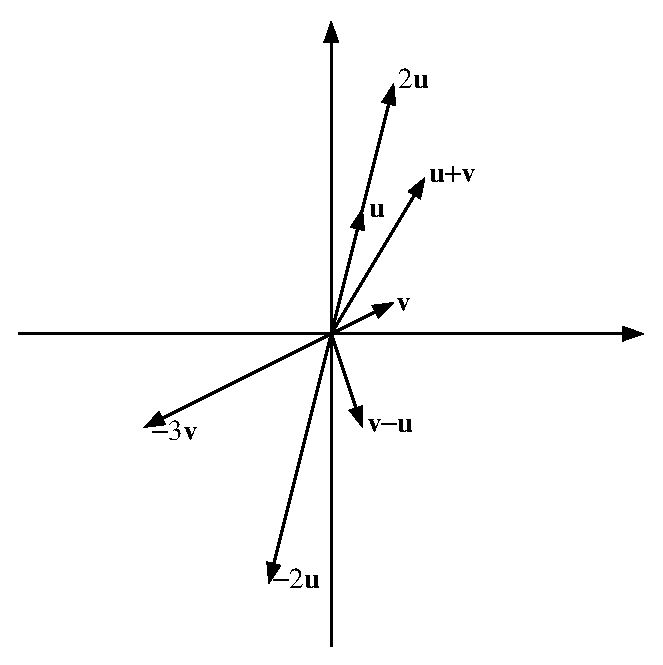
\includegraphics{figures/9_2_Act_5_Vectors_a}} \ \ \resizebox{!}{2.25in}{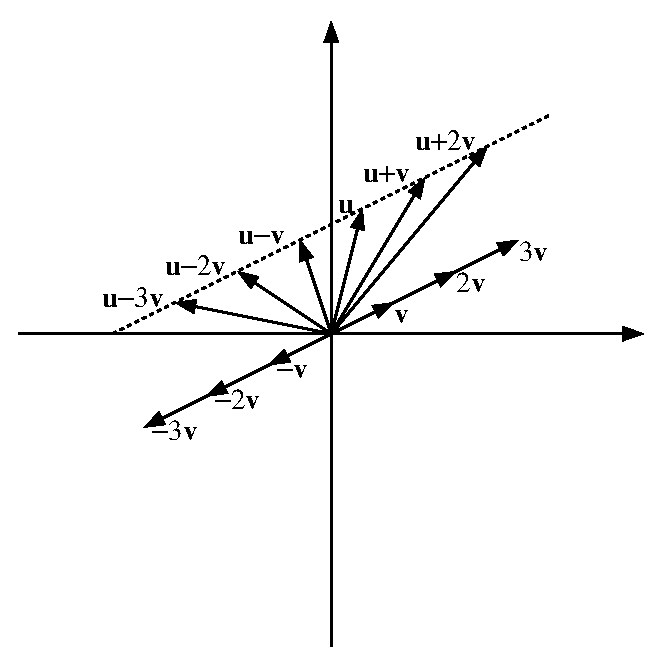
\includegraphics{figures/9_2_Act_5_Vectors_b}}
      \end{center}
     \item As the figure in part (e) illustrates, this is a line through the terminal point of the vector $\vu$ in standard position in the direction of the vector $\vv$. 
	\ea
\end{activitySolution}
\aftera


\subsection*{The Magnitude of a Vector}

By definition, vectors have both direction and magnitude (or
length). We now investigate how to calculate the magnitude
of a vector.  Since a vector $\vv$ can be represented
by a directed line segment, we can use the distance formula to
calculate the length of the segment. This length is the
\emph{magnitude} of the vector $\vv$ and is denoted $|\vv|$.

\begin{activity} \label{A:9.2.7}

\begin{figure}[h]
\begin{center}
\begin{minipage}{3in}
\begin{center}
%\resizebox{!}{2.25in}{\includegraphics{figures/9_2_Vector_magnitude1}}
\includegraphics{figures/fig-9-20.eps}
\end{center}
\caption{The vector defined by $A$ and $B$.} %$\overrightarrow{AB}$.
\label{F:9.2.vector_magnitude}
\end{minipage}
\begin{minipage}{3in}
\begin{center}
%\resizebox{!}{2.25in}{\includegraphics{figures/9_2_Vector_magnitude2}}
\includegraphics{figures/fig-9-21.eps}
\end{center}
\caption{An arbitrary vector, $\vv$.}
\label{F:9.2.vector_magnitude2}
\end{minipage}
\end{center}
\end{figure}
	\ba
	\item Let $A = (2,3)$ and $B = (4,7)$, as shown in Figure \ref{F:9.2.vector_magnitude}. Compute $|\overrightarrow{AB}|$.


	\item Let $\vv = \langle v_1, v_2 \rangle$ be the vector in $\R^2$ with components $v_1$ and $v_2$ as shown in Figure \ref{F:9.2.vector_magnitude2}. Use the distance formula to find a general formula for $|\vv|$.


	\item Let $\vv = \langle v_1, v_2, v_3 \rangle$ be a vector in $\R^3$. Use the distance formula to find a general formula for $|\vv|$.

        \item Suppose that $\vu = \langle 2,3\rangle$ and $\vv =
          \langle -1,2\rangle$.  Find $|\vu|$, $|\vv|$, and
          $|\vu+\vv|$.  Is it true that $|\vu + \vv| = |\vu|+|\vv|$?

        \item Under what conditions will $|\vu+\vv| = |\vu|+|\vv|$? (Hint: Think about how $\vu$, $\vv$, and $\vu+\vv$ form the sides of a triangle.)

        \item With the vector $\vu = \langle 2,3\rangle$, find the
          lengths of $2\vu$, $3\vu$, and $-2\vu$, respectively, and use proper notation to label your results.  

        \item If $t$ is any scalar, how is $|t\vu|$
          related to $|\vu|$?

        \item A {\bf unit vector} is a vector whose magnitude is 1.
          Of the vectors ${\bf i}$, ${\bf j}$, and ${\bf i} + {\bf
            j}$, which are unit vectors?

        \item Find a unit vector $\vv$ whose direction is the same as
          $\vu = \langle 2, 3\rangle$. (Hint: Consider the result of part (g).)


	\ea


\end{activity}
\begin{smallhint}

\end{smallhint}
\begin{bighint}

\end{bighint}
\begin{activitySolution}
\ba
	\item In this case we have $\overrightarrow{AB} = \langle 2,4\rangle$, so 
\[|\overrightarrow{AB}|  = \sqrt{2^2+4^2} = \sqrt{20}.\]
	\item The distance formula tells us that 
\[|\vv| = \sqrt{v_1^2 + v_2^2}.\]
	\item The distance formula tells us that 
\[|\vv| = \sqrt{v_1^2 + v_2^2+v_3^2}.\]
    \item We have $|\vu| = \sqrt{13}$, $|\vv| = \sqrt{5}$, while $|\vu+\vv| = |\langle 1,5\rangle| = \sqrt{26}$. So $|\vu + \vv| \neq |\vu|+|\vv|$.
    \item Since $\vu$, $\vv$, and $\vu+\vv$ form the sides of a triangle, and $\vu+\vv$ provides a straight path from the tail of $\vu$ to the tip of $\vv$, the length of $\vu+\vv$ should be longer that the sum of the lengths of the other sides, unless $\vu$ and $\vv$ are on the same ray. 
     \item In this case we have 
\begin{align*}
|2\vu| &= |\langle 4,6 \rangle | = \sqrt{52} \\
|3\vu| &= |\langle 6,9 \rangle | = \sqrt{117} \\
|-2\vu| &= |\langle -4,-6 \rangle | = \sqrt{52} \\
\end{align*}
    \item Note that if $\vu = \langle u_1, u_2\rangle$, then 
\[|t\vu| = |\langle tu_1, tu_2 \rangle | = \sqrt{t^2u_1^2 + t^2u_2^2} = \sqrt{t^2}\sqrt{u_1^2+u_2^2} = |t||\vu|.\]
This same argument applies in any dimension, so we conclude that 
\[|t\vu| = |t||\vu|.\]
    \item Since $|{\bf i}| = |\langle 1,0 \rangle | = 1$, $|{\bf j}| = |\langle 0,1 \rangle | = 1$, and $|{\bf i }+ {\bf j}| = |\langle 1,1 \rangle | = \sqrt{2}1$, we see that only ${\bf i}$ and ${\bf j}$ are unit vectors. 
     \item As we saw earlier, 
\[|t\vu| = |t||\vu|,\]
So 
\[\left| \frac{1}{|\vu|} \vu \right| = \frac{1}{|\vu|} |\vu| = 1.\]
Therefore, the vector $\frac{1}{13} \langle 2,3\rangle$ is a unit vector in the direction of $\vu = \langle 2, 3\rangle$.
	\ea
\end{activitySolution}
\aftera



% We close this section with an important definition.

% \vspace*{5pt}
% \nin \framebox{\hspace*{3 pt}
% \parbox{6.25 in}{\begin{definition} A \textbf{unit vector}\index{unit vector} is a vector with magnitude or length 1. \end{definition}
% } \hspace*{3 pt}}
% \vspace*{5pt}

% As we will see in subsequent work, unit vectors\index{unit vector}
% will be important for defining the direction of a vector and
% projections of vectors.

%\begin{activity} \label{A:9.2.8}

    \ba
    \item Let $\vv = \langle 1,2 \rangle$ in $\R^2$. What is the length of $\vv$? Use the length of $\vv$ to find a unit vector that is parallel to $\vv$.


    \item Let $\vv$ be an arbitrary nonzero vector in $\R^3$. Write a general formula for a unit vector that is parallel to $\vv$.


    \ea


\end{activity}
\begin{smallhint}

\end{smallhint}
\begin{bighint}

\end{bighint}
\begin{activitySolution}

\end{activitySolution}
\aftera



%\nin \framebox{\hspace*{3 pt}
%\parbox{6.25 in}{
\begin{summary}
\item A vector is any object that possesses the attributes of
  magnitude and direction. Examples of vector quantities are position,
  velocity, acceleration, and force.  
\item Two vectors are equal if they have the
  same direction and magnitude. Notice that position is not considered, so a vector is independent of its location.
\item If $\vu = \langle u_1, u_2, \ldots, u_n \rangle$ and $\vv =
  \langle v_1, v_2, \ldots, v_n \rangle$ are two vectors in $\R^n$,
  then their vector sum is the vector
\[\vu + \vv = \langle u_1+v_1, u_2+v_2, \ldots, u_n+v_n \rangle.\]
If $\vu = \langle u_1, u_2, \ldots, u_n \rangle$ is a vector in $\R^n$
and $c$ is a scalar, then the scalar multiple $c\vu$ is the vector
 \[c\vu = \langle cu_1, cu_2, \ldots, cu_n \rangle.\]
\item The magnitude of the vector $\vv = \langle v_1, v_2, \ldots, v_n
  \rangle$ in $\R^n$ is the scalar
  \[|\vv| = \sqrt{v_1^2+v_2^2+ \cdots + v_n^2}.\] A vector $\vu$ is a
  unit vector provided that $|\vu| = 1$. If $\vv$ is a nonzero vector,
  then the vector $\frac{\vv}{|\vv|}$ is a unit vector with the same
  direction as $\vv$.
\end{summary}
%} \hspace*{3 pt}}

\nin \hrulefill

\begin{exercises} 

\item \label{Ez:9.2.1}   Let $\vv = \langle 1, -2 \rangle$, $\vu = \langle 0, 4 \rangle$, and $\vw = \langle -5, 7 \rangle$.
%\begin{figure}[h]
%\begin{center}
 %\includegraphics{figures/1_1_Ez1.eps}
 %\caption{A bungee jumper's height function.} \label{F:1.1.Ez1}
%\end{center}
%\end{figure}

    \ba
    	\item Determine the components of the vector $\vu - \vv$.
        \item Determine the components of the vector $2\vv - 3\vu$.
        \item Determine the components of the vector $\vv + 2\vu - 7 \vw$.
        \item Determine scalars $a$ and $b$ such that $a \vv + b\vu = \vw.$
    \ea

\begin{exerciseSolution}
    \ba
    	\item In this example we have $\vu - \vv = \langle 0-1, 4-(-2) \rangle = \langle -1, 6 \rangle$.
        \item In this example we have $2\vv - 3\vu = \langle 2(1)-3(0), 2(-2)-3(4) \rangle = \langle 2, -16 \rangle$.
        \item In this example we have $\vv + 2\vu - 7 \vw = \langle 1+2(0)-7(-5), -2+2(4)-7(7) \rangle = \langle 36, -43 \rangle$.
        \item Since $a \vv + b\vu = \langle a, -2a+4b \rangle$, in order for $a \vv + b\vu$ to equal $\vw$ we must have $a=-5$ and $-2(-5)+4b = 7$. So $a=-5$ and $b = -\frac{3}{4}$.  
    \ea
\end{exerciseSolution}


\item \label{Ez:9.2.2}  Let $\vu = \langle 2, 1 \rangle $ and $\vv = \langle 1, 2 \rangle$.


    \ba
    \item Determine the components and draw geometric representations of the vectors $2\vu$, $\frac{1}{2}\vu$, $(-1)\vu$, and $(-3)\vu$ on the same set of axes.

    \item Determine the components and draw geometric representations of the vectors $\vu + \vv$, $\vu + 2\vv$, and $\vu + 3\vv$.
    
    \item Determine the components and draw geometric representations of the vectors $\vu - \vv$, $\vu - 2\vv$, and $\vu - 3\vv$.
    
    \item Recall that $\vu - \vv = \vu + (-1)\vv$.  Use the ``tip to tail'' perspective for vector addition to explain why the difference $\vu - \vv$ can be viewed as a vector that points from the tip of $\vv$ to the tip of $\vu$.
    
   
    \ea

\begin{exerciseSolution}
    \ba
    \item Here we have 
\begin{align*}
2\vu &= \langle 4,2 \rangle \\
\frac{1}{2}\vu &= \left\langle 1, \frac{1}{2} \right\rangle \\
(-1)\vu	&= \langle -2, -1 \rangle \\
(-3)\vu &= \langle -6, -3 \rangle.
\end{align*}
Pictures of these vectors, all of which lie on the same line, are shown in the figure below. 
\begin{center}
\resizebox{!}{2.0in}{\includegraphics{9_2_Ex_2_a}}
%\includegraphics{figures/9_2_Ex_2_a}
\end{center}


    \item Here we have 
\begin{align*}
\vu + \vv &= \langle 3,3 \rangle \\
\vu + 2\vv &= \langle 4, 5 \rangle \\
\vu + 3\vv	&= \langle 5, 7 \rangle.
\end{align*}
Pictures of these vectors, whose terminal points all lie on the same line, are shown in the figure below. 
\begin{center}
\resizebox{!}{2.0in}{\includegraphics{9_2_Ex_2_b}}
\end{center}
    
    \item Here we have 
\begin{align*}
\vu - \vv &= \langle 1,-1 \rangle \\
\vu - 2\vv &= \langle 0, -3 \rangle \\
\vu - 3\vv	&= \langle -1, -5 \rangle.
\end{align*}
Pictures of these vectors, whose terminal points all lie on the same line, are shown in the figure below. 
\begin{center}
\resizebox{!}{2.0in}{\includegraphics{9_2_Ex_2_c}}
\end{center}

   
    \item The figure below illustrates that $\vu - \vv = \vu + (-1)\vv$ is the same as the vector from the tip of $\vv$ to the tip of $\vu$.
\begin{center}
\resizebox{!}{2.0in}{\includegraphics{9_2_Ex_2_d}}
\end{center}   
   
    \ea
\end{exerciseSolution}


\item \label{Ez:9.2.3}  Recall that given any vector $\vv$, we can calculate its length, $|\vv|$.  Also, we say that two vectors that are scalar multiples of one another are \emph{parallel}. 


    \ba
    \item Let $\vv = \langle 3,4 \rangle$ in $\R^2$.  Compute $|\vv|$, and determine the components of the vector $\vu = \frac{1}{|\vv|} \vv$.  What is the magnitude of the vector $\vu$?  How does its direction compare to $\vv$?
    
    \item Let $\vw = 3\vi - 3\vj$ in $\R^2$.  Determine a unit vector $\vu$ in the same direction as $\vw$.
    
    \item Let $\vv = \langle 2, 3, 5 \rangle$ in $\R^3$.  Compute $|\vv|$, and determine the components of the vector $\vu = \frac{1}{|\vv|} \vv$.  What is the magnitude of the vector $\vu$?  How does its direction compare to $\vv$?

    \item Let $\vv$ be an arbitrary nonzero vector in $\R^3$. Write a general formula for a unit vector that is parallel to $\vv$.

    \ea

\begin{exerciseSolution}
    \ba
     \item We know that $|\vv| = \sqrt{3^2+4^2} = 5$. So $\vu = \frac{1}{|\vv|} \vv = \left\langle \frac{3}{5}, \frac{4}{5} \right\rangle$. The magnitude of $\vu$ is $|\vu| = \sqrt{\left(\frac{3}{5}\right)^2 + \left(\frac{4}{5}\right)^2} = 1$. Since $\vu$ is a positive scalar multiple of $\vv$, the vector $\vu$ is a unit vector in the direction of $\vv$. 
    
    \item As in part (a), to find a unit vector in the direction of $\vw$, we divide $\vw$ by its magnitude. So a unit vector $\vu$ in the same direction as $\vw$ is $\vu = \frac{1}{|\vw|} \vw = \frac{1}{\sqrt{18}} \vw = \left\langle \frac{3}{\sqrt{18}}, -\frac{3}{\sqrt{18}} \right\rangle$.
    
    \item We know that $|\vv| = \sqrt{2^2+3^2+5^2} = \sqrt{38}$. So $\vu = \frac{1}{|\vv|} \vv = \left\langle \frac{2}{\sqrt{38}}, \frac{3}{\sqrt{38}}, \frac{5}{\sqrt{38}} \right\rangle$. The magnitude of $\vu$ is $|\vu| = \sqrt{\left(\frac{2}{\sqrt{38}}\right)^2  + \left(\frac{3}{\sqrt{38}}\right)^2 + \left(\frac{5}{\sqrt{38}}\right)^2} = 1$. Since $\vu$ is a positive scalar multiple of $\vv$, the vector $\vu$ is a unit vector in the direction of $\vv$. 

    \item If $\vv$ is an arbitrary nonzero vector in $\R^3$, then the vector $\frac{1}{|\vv|} \vv$ is a unit vector that is parallel to $\vv$.

    \ea
\end{exerciseSolution}

\end{exercises}

\afterexercises


\clearpage
